% =============================================================================
% Section 4.10: Discussion and Q&A Module
% =============================================================================

\section{Discussion and Q\&A Module}
\label{sec:discussion-module}

\subsection{Thread and Post Aggregate Design}

The Discussion module implements a tree-structured thread-and-post model common to forum and Q\&A systems. The aggregate root is \texttt{ThreadEntity}, which is scoped to a specific lesson (per-lesson discussion) or to a course (general discussion). A thread has a title, a creator (learner or instructor), a collection of \texttt{PostEntity} children, and a lifecycle status.

The aggregate enforces the forum structure invariants:

\begin{lstlisting}[caption=Discussion Thread Aggregate,label=lst:thread-aggregate]
export class ThreadEntity {
  constructor(
    public readonly id: string,
    public readonly courseId: string,
    public readonly lessonId: string | null,
    public readonly creatorId: string,
    public title: string,
    public body: string,
    public isPinned: boolean,
    public isResolved: boolean,
    public isHidden: boolean,
    public posts: PostEntity[],
    public createdAt: Date,
    public updatedAt: Date,
  ) {}

  addPost(learnerId: string, body: string): PostEntity {
    if (this.isHidden)
      throw new BusinessRuleViolation('Thread is closed');
    if (body.length > 5000)
      throw new BusinessRuleViolation('Post exceeds 5000 characters');

    const post = PostEntity.create({
      threadId: this.id,
      authorId: learnerId,
      body,
    });

    this.posts.push(post);
    this.updatedAt = new Date();
    return post;
  }

  markResolved(): void {
    this.isResolved = true;
    this.updatedAt = new Date();
  }
}
\end{lstlisting}

When a post is added by an instructor to a learner's thread, the \texttt{InstructorReplied} domain event is published. This event is consumed by the Notifications module, which sends an email notification to the thread creator. The notification includes a direct link to the thread in the learner dashboard.

\subsection{Instructor Reply Notifications}

Notification flow: \texttt{ThreadEntity.addPost()} creates a \texttt{PostEntity} and marks the thread as updated. The \texttt{AddPostUseCase} persists the thread and post, then publishes an outbox event. The Notifications module's event handler checks whether the author of the new post has the \texttt{instructor} role on the course. If so, it creates a \texttt{Notification} entity for each learner who has posted in the thread, containing the instructor's reply excerpt and a link to the thread. Notifications are delivered via Resend transactional email and are also accessible via the NexaLearn REST API for in-app notification display.

Figure~\ref{fig:discussion-statemachine} illustrates the thread lifecycle using boolean flags: a thread is open by default, marked as resolved by the instructor, or hidden through moderation.

\begin{figure}[H]
  \centering
  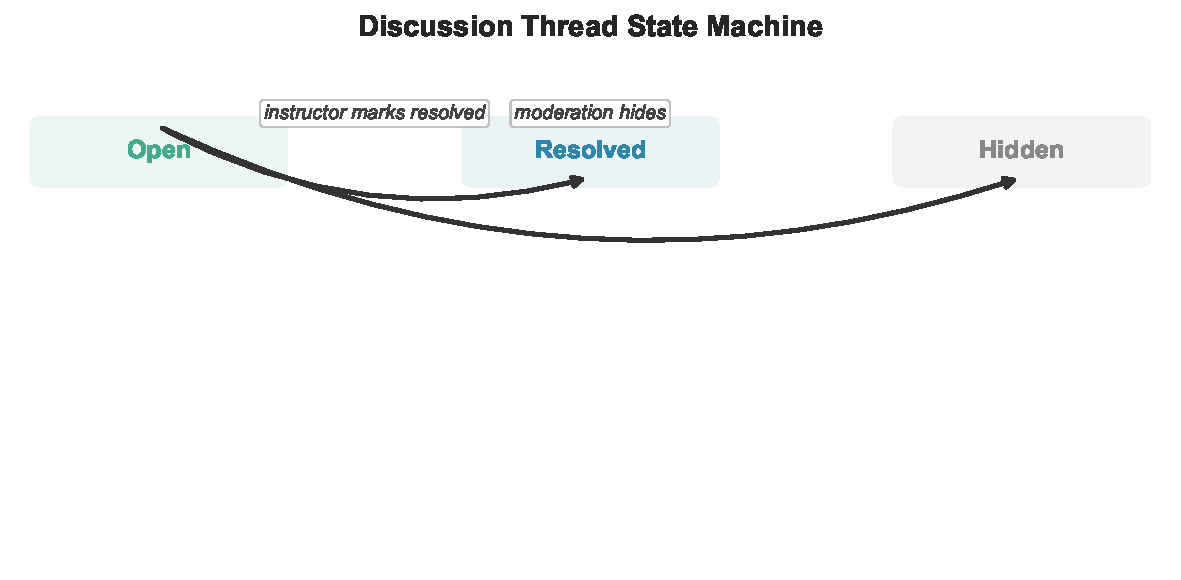
\includegraphics[width=0.5\textwidth]{images/statemachines/discussion_statemachine.pdf}
  \caption{Discussion Thread State Machine}
  \label{fig:discussion-statemachine}
\end{figure}
